
%\documentstyle[epsf,twocolumn]{jarticle}       %LaTeX2e仕様
% \documentclass[twocolumn]{jarticle}     %pLaTeX2e仕様(platex.exeの場合)
\documentclass[onecolumn]{ujarticle}   %pLaTeX2e仕様(uplatex.exeの場合)
%%%%%%%%%%%%%%%%%%%%%%%%%%%%%%%%%%%%%%%%%%%%%%%%%%%%%%%%%%%%%%
%%
%%  基本バージョン
%%
%%%%%%%%%%%%%%%%%%%%%%%%%%%%%%%%%%%%%%%%%%%%%%%%%%%%%%%%%%%%%%%%
\setlength{\topmargin}{-45pt}
%\setlength{\oddsidemargin}{0cm}
\setlength{\oddsidemargin}{-7.5mm}
%\setlength{\evensidemargin}{0cm}
\setlength{\textheight}{24.1cm}
%setlength{\textheight}{25cm}
\setlength{\textwidth}{17.4cm}
%\setlength{\textwidth}{172mm}
\setlength{\columnsep}{11mm}

%\kanjiskip=.07zw plus.5pt minus.5pt


% 【節が変わるごとに (1.1)(1.2) … (2.1)(2.2) と数式番号をつけるとき】
%\makeatletter
%\renewcommand{\theequation}{%
%\thesection.\arabic{equation}} %\@addtoreset{equation}{section}
%\makeatother

%\renewcommand{\arraystretch}{0.95} 行間の設定
%%%%%%%%%%%%%%%%%%%%%%%%%%%%%%%%%%%%%%%%%%%%%%%%%%%%%%%%
%\usepackage{graphicx}   %pLaTeX2e仕様(\documentstyle ->\documentclass)
\usepackage[dvipdfmx]{graphicx}
\usepackage{subcaption}
\usepackage{multirow}
\usepackage{amsmath}
\usepackage{url}
\usepackage{ulem}
\usepackage{algorithm}
\usepackage{algorithmic}
\usepackage{listings} %,jlisting} %日本語のコメントアウトをする場合jlistingが必要
%ここからソースコードの表示に関する設定
\lstset{
  basicstyle={\ttfamily},
  identifierstyle={\small},
  commentstyle={\smallitshape},
  keywordstyle={\small\bfseries},
  ndkeywordstyle={\small},
  stringstyle={\small\ttfamily},
  frame={tb},
  breaklines=true,
  columns=[l]{fullflexible},
  numbers=left,
  xrightmargin=0zw,
  xleftmargin=3zw,
  numberstyle={\scriptsize},
  stepnumber=1,
  numbersep=1zw,
  lineskip=-0.5ex
}
\newcommand{\argmax}{\mathop{\rm arg~max}\limits}
\newcommand{\argmin}{\mathop{\rm arg~min}\limits}

%%%%%%%%%%%%%%%%%%%%%%%%%%%%%%%%%%%%%%%%%%%%%%%%%%%%%%%%
\begin{document}

	%bibtex用の設定
	%\bibliographystyle{ujarticle}

	% \twocolumn[
		\noindent
		\hspace{1em}
		2022 年 8 月 12 日
		ゼミ資料
		\hfill
		杉山 竜弥
		\vspace{2mm}

		\hrule
		\begin{center}
			{\Large \bf 進捗報告}
		\end{center}
		\hrule
		\vspace{9mm}
	% ]


\section{今週やったこと}
\begin{itemize}
  \item データセットの許可メール
  \item 使用するモデルの検討.
\end{itemize}


\section{メールの結果}
サイトの運営者より使用許可を頂きました.
大阪公立大学高専 (美術担当) の方とのことです.

得られた許可:画像・文章・曲・動画

% 杉山竜弥さま
%
% えかきうた作者の西村です。
% 研究でのご使用の件、了解しました。どうぞご自由にお使い下さい。
%
% 私も学校で教えていますので、研究にご協力でき、うれしく思います。
% サイトやYoutubeから、必要なものをダウンロード下さい。
% 他に必要なデータなどがありましたら、ご連絡を
% ~
% goma.simsim@gmail.com
%
% ところで、教えている学校は、大阪公立大学高専(担当は美術)です。奇遇ですね。
%
% ご研究の概要など、差し支えない範囲でお教え頂ければ幸いです。
% また外部発表の機会には、ぜひお声かけください。
% よろしくお願いいたします。
%
% 西村有理
% ---
% コマ撮り人形アニメ OPEN the SESAME
% goma@to.email.ne.jp
% goma.simsim@gmail.com

\section{データセットの整形}
イラストに含まれる枠が学習の妨げになりそうなので,
枠なしバージョンも生成した.
若干線のアンチエイリアスが変化したがそこまで大きな問題ではないと思われる.


\begin{figure}[htbp]
    \begin{tabular}{cc}
      \begin{minipage}[t]{0.45\hsize}
        \centering
        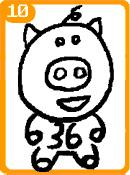
\includegraphics[keepaspectratio, height=30mm]{buta_.jpg}
        \caption{変換前}
        \label{fig:result2_1}
      \end{minipage} &
      \begin{minipage}[t]{0.45\hsize}
        \centering
        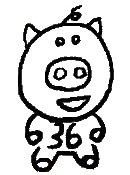
\includegraphics[keepaspectratio, height=30mm]{buta.jpg}
        \caption{変換後}
        \label{fig:result2_2}
      \end{minipage}
      \\\\
      \begin{minipage}[t]{0.45\hsize}
        \centering
        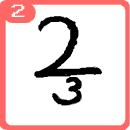
\includegraphics[keepaspectratio, height=30mm]{ahiru_.jpg}
        \caption{変換前}
        \label{fig:result2_1}
      \end{minipage} &
      \begin{minipage}[t]{0.45\hsize}
        \centering
        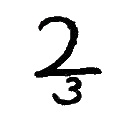
\includegraphics[keepaspectratio, height=30mm]{ahiru.jpg}
        \caption{変換後}
        \label{fig:result2_2}
      \end{minipage} \\
    \end{tabular}
  \end{figure}

\section{問題設定}
このデータセットを利用する問題をいくつか考えた.

\begin{itemize}
  \item 順序推定
  \item 絵描き歌のクラス推定
  \item 最終状態の予測
\end{itemize}

順序推定はいちばん簡単な問題として,画像や文章を様々な順序で入力し正順かどうかを判定する問題.

クラス推定は単純に画像と文章の列を入力し描かれたもののクラスを推定する問題であるが,
このデータセットは 1 クラスにつき 1 つのデータしか存在しないため
これをテストデータに使うと 0-shot での推定となりかなり困難であると思われる.

最終状態の予測は最後以外の画像や文章を入力し,最後の画像や文章を予測させる問題.

\subsection{モデルの調査}

どの問題を解くにしても必要な,画像の時系列データ(動画)を入力とするモデルを調べたところ,
似たモデルが同時期に複数提案されていることが分かったため,
まず Video Vision Transformer (ViViT) を使用できるようにした.
実装と事前学習パラメータも使用できることを確認した.

次に必要なのは自前のデータセットを ViViT の入力形式に変換することである.

% 入力:画像,文章の時系列データ
% 出力:順序判定,次の画像生成,文章生成,画像列から文章の推定,文章列からクラス推定
%
% 難易度順
% 1. 順序判定
% 1. 文章列からクラス推定
% 1. 画像列 (2~n枚) から文章の推定
% 1. 次の画像 or 文章生成
%
% 動画モデル
% Video Transformer Network (2021)
% Is Space-Time Attention All You Need for Video Understanding? (2021)
% An Image is Worth 16×16 Words, What is a Video Worth? (2021)
% ViViT: A Video Vision Transformer (2021)
%
% 動画キャプション生成モデルが最も近い?
%
% 動画モデル:時間がかかる...
%
% あるクラスに対してデータが1つしかない
%
% ViViTをやってみる→ViTを動かす?
% パラメータはゲット(ViViTとViT共通?)
%
% データセット:一部だが1セットくらい入れてみたい


\section{予定}
\begin{itemize}
  \item ViViT の予備実験
\end{itemize}


% \begin{figure}[h]
%   \begin{center}
%     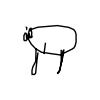
\includegraphics[clip,width=20mm]{decode1.png}
%     \caption{比較元のデコードスケッチ}
%     \label{fig:result2_1}
%   \end{center}
% \end{figure}

% 参考文献リスト
% \bibliographystyle{unsrt}
% \bibliography{ref}
\end{document}
